\documentclass[fsharpNotes.tex]{subfiles}
\graphicspath{ {./figures/} }

\begin{document}
\chapter{Making Programs and Documenting Them}

\abstract{
  Programs are more than a set of instructions, which when executed pro- duces the desired result. Programming is an activity, and a program is the result of a process, in which a problem has been expressed, analyzed, subdivided, implemented, tested, and possibly rephrased. And often the process and its result are to be wrapped and documented for it to be useful by the programmer or others. In this chapter, we will zoom out, and focus on some of these surrounding processes. The chapter will describe: 
  \begin{itemize}
  \item How to design functions.
  \item How and why to document programs using in-code documentation.
  \end{itemize}
}

\section{The 8-step Guide to Writing Functions}
\label{sec:8step}
Pólya's problem solving technique described in \Cref{sec:howToSolveProblems} is a useful starting point for solving problems, and for the object-oriented programming paradign to be discussed in later chapters \Cref{chap:oopp}, approaches such as Pólya's have been put into systems. Regardless of the origin, there is always a point, where a programmer has to focus on small scale problems such as: Which functions, should be used, and how should the functions be designed? This is not an area heavily investigated in the literature, but often a skill that programmers pick up by activily engaging in programming alone or with other programmers. However, here I will venture a recipes for designing functions, which me and my collagues call The 7-step guide to writing functions. It is not meant as the ultimate guide or as required steps, but it is our experience that these steps contain essential elements that consiously or perhaps unconsioulsy always take part in designing useful and resuable functions.

To decide which functions to write and how to write them:
\begin{enumerate}
\item Note: Write a short note on what a function should do.
\item Name: Invent a name for the function. Semantically meaningful names should be preferred.
\item External test: Write a small test-program, which uses the yet to be written function.
\item Type: Decide what type, the function should have, e.g., by how you used it in your test-program.
\item Implement: Write the function and possibly its helper functions.
\item Internal test: Extend your test-program with more examples, where you use the function and based on its implementation.
\item Run: Run the test-program
\item Document: Write a brief in-code documentation of the function, see \Cref{chap:documentation}.
\end{enumerate}

As an example, let us revisit the problem of solving a quadratic equation: The task is to find the zero-crossings of a second degree polynomial, i.e., $f(x)=ax^2+bx+c=0$. The process could be as follows:
\begin{enumerate}
\item Note: We decide to stick to the mathematical description:
  \begin{quote}
    Given parameters $a$, $b$, and $c$, the function should return the 0, 1, or possibly 2 locations $x$, where $f(x)=0$.
  \end{quote}
\item Name: This function may be used together with solvers for other equations, so we decide to give it the rather long name
  \begin{quote}
    \lstinline{solveQuadraticEquation}.
  \end{quote}
\item External test: We decide to a single tests to get a feeling of how the function is to be used:
\begin{codeNOutput}[label=solveQuadraticEquationTest,
  top=-5pt,
  bottom=-5pt,
  left=-2pt,
  right=-2pt,
]{: Defining the function \lstinline{sum}}
\begin{lstlisting}
let p = solveQuadraticEquation 1.0 0.3 -1.0
printfn "0=1.0x^2+0.3x-1.0 => x = %1" p;;
\end{lstlisting} 
\end{codeNOutput}
\item Type: Since there may be 0-2 points $x$, where $f(x)=0$, the output answers could be a tuple. Furhter, since $a,b,c,x\in\Re$, we will use floats. Hence,
  \begin{quote}
    \lstinline{solveQuadraticEquation -> float -> float -> float -> float*float}.
  \end{quote}
\item Implement: Thinking about how to write  \lstinline{solveQuadraticEquation}, we decide that since the calculation of the discriminant is done twice, we will add it as a helper function. Our resulting code is:
\begin{codeNOutput}[label=solveQuadraticEquationImplementation,
  top=-5pt,
  bottom=-5pt,
  left=-2pt,
  right=-2pt,
]{: Defining the function \lstinline{sum}}
\begin{lstlisting}
let discriminant a b c = b ** 2.0 - 4.0 * a * c

let solveQuadraticEquation a b c =
  let d = discriminant a b c
  ((-b + sqrt d) / (2.0 * a),
   (-b - sqrt d) / (2.0 * a))
\end{lstlisting}
\end{codeNOutput}
\item Internal test: Working with the code, we realize that it is unclear, what happens, when there are 0 og 1 solutions, so we update the external test and add more tests:
\begin{codeNOutput}[label=solveQuadraticEquationTest,
  top=-5pt,
  bottom=-5pt,
  left=-2pt,
  right=-2pt,
]{: Defining the function \lstinline{sum}}
\begin{lstlisting}
let p1 = solveQuadraticEquation 1.0 0.3 -1.0
printfn "0=1.0x^2+0.3x-1.0 => x = %A" p1
let p2 = solveQuadraticEquation 1.0 0.0 0.0
printfn "0=1.0x^2+0.3x-1.0 => x = %A" p2
let p3 = solveQuadraticEquation 1.0 0.0 1.0
printfn "0=1.0x^2+0.3x-1.0 => x = %A" p3
\end{lstlisting} 
\end{codeNOutput}
\item Run: The compelete code with examples and its output, when executed is shown in \Cref{solveQuadraticEquation}
  \fs{solveQuadraticEquation}{Solving quadratic equations}
\item Document: The following section will discuss how to perform in-code documentation and use \Cref{solveQuadraticEquation} as an example.
\end{enumerate}


\section{Programming as a Commication Activity}
\label{chap:documentation}
Documentation is a very important part of writing programs, since it is most unlikely that you will be writing really obvious code. Moreover, what seems obvious at the point of writing may be mystifying months later to the author and to others. Documentation serves several purposes:
\begin{enumerate}
\item Communicate to the user of the code, what it does and how to use it. In this book, we will emphasize the XML-standard for this purpose.
\item Highlight big insights essential for the code, which is important for other programmers to understand and maintain the code.
\item Highlight possible conflicts and/or areas where the code could be changed later, which is also targeted programmers rather than users of the code.
\end{enumerate}
The essential point is that coding is a journey in problem-solving, and proper documentation is an aid in understanding the solution and the journey that lead to it. Documentation is most often a mixture of in-code documentation and accompanying documents. Here, we will focus on in-code documentation which arguably causes problems in multi-language environments and run the risk of bloating code. Since documentation is about human-to-human communication, there is no correct documentation. However, as in all things the documentation can both be too little and too much, and the ability to produce documentation is best learned by example and by doing.

F\# has two different syntaxes for comments. Comments can be block
comments: \jon{color of '*' is wrong.}
%
\begin{verbatimwrite}{\ebnf/blockComment.ebnf}
(**<*any text*>**)
\end{verbatimwrite}
\syntax{\ebnf/blockComment.ebnf}{Block comments.\idxss{(**)@\lstinline{(**)}}}
%
The comment text \lstinline[language=syntax]{(*<*any text*>*)} can be any text and is stilled parsed by F\# as keywords and basic types, implying that \lstinline!(* a comment (* in a comment *) *)! and \lstinline[morecomment={[l][\color{commentsColor}]{(*}}]!(* "*)" *)! are valid comments, while \lstinline!(* " *)! is invalid.

Alternatively, comments may also be line comments,
%
\begin{verbatimwrite}{\ebnf/lineComment.ebnf}
//<*any text*>
\end{verbatimwrite}
\syntax{\ebnf/lineComment.ebnf}{Line comments.\idxss{//@\lstinline{//}}}
%
where the comment text ends after the first newline.

The block and line comments are used principally for communicating insights and comments into the code between programmers which want to understand and/or maintain the code. 

Users of the code, are most likely also programmers but have an outside perspective. They are more interested in what the code does, and how it is to be used. For this we recommend the \idx{Extensible Markup Language} documentation standard (\idx{XML-standard}) \footnote{For specification of C\# documentations comments see ECMA-334: \url{http://www.ecma-international.org/publications/files/ECMA-ST/Ecma-334.pdf}}. All lines of the XML-standard starts with a triple-slash \lstinline{///}. Thus, it is a line-comment, where an extra slash has been added for visual flair. XML consists of tags which always appear in pairs, e.g., the tag ``tag'' would look like \lstinline[language=xml]!<tag> ... </tag>!. A subset of tags are listed in \Cref{tab:xmlTags}.
\begin{table}
  \centering
  \rowcolors{2}{oddRowColor}{evenRowColor}
  \begin{tabularx}{\linewidth}{|l|X|}
       \hline
    \rowcolor{headerRowColor} Tag & Description\\
    \hline
    \lstinline[language=xml]!<c>! &Set text in a code-font.\\
    \hline
    \lstinline[language=xml]!<code>! &Set one or more lines in code-font.\\
    \hline
    \lstinline[language=xml]!<example>! &Set as an example.\\
    \hline
    \lstinline[language=xml]!<exception>! &Describe the exceptions a function can throw.\\
    \hline
    \lstinline[language=xml]!<list>! &Create a list or table.\\
    \hline
    \lstinline[language=xml]!<para>! &Set text as a paragraph.\\
    \hline
    \lstinline[language=xml]!<param>! &Describe a parameter for a function or constructor.\\
    \hline
    \lstinline[language=xml]!<paramref>! &Identify that a word is a parameter name.\\
    \hline
    \lstinline[language=xml]!<permission>! &Document the accessibility of a member.\\
    \hline
    \lstinline[language=xml]!<remarks>! &Further describe a function.\\
    \hline
    \lstinline[language=xml]!<returns>! &Describe the return value of a function.\\
    \hline
    \lstinline[language=xml]!<see>! &Set as link to other functions.\\
    \hline
    \lstinline[language=xml]!<seealso>! &Generate a See Also entry.\\
    \hline
    \lstinline[language=xml]!<summary>! &Main description of a function or value.\\
    \hline
    \lstinline[language=xml]!<typeparam>! &Describe a type parameter for a generic type or method.\\
    \hline
    \lstinline[language=xml]!<typeparamref>! &Identify that a word is a type parameter name.\\
    \hline
    \lstinline[language=xml]!<value>! &Describe a value.\\
    \hline
  \end{tabularx}
  \caption{Recommended XML tags for documentation comments, from ECMA-334 3rd Edition, Annex E, Section 2.}
  \label{tab:xmlTags}
\end{table}
If no tags are used, then it is automatically assumed to be a \lstinline[language=xml]!<summary>!. An example of a documented script is shown in \Cref{commentExample}.
is:
%
\fsCode{commentExample}{commentExample}{Code with XML comments.}{}
%

\begin{comment}
Mono's \lstinline[language=console]{fsharpc} command may be used to extract the comments into an XML file, as demonstrated in \Cref{convertingToXML}.
\begin{codeNOutput}[label=convertingToXML]{, Converting in-code comments to XML.}
  \begin{lstlisting}[language=console]
$ fsharpc --doc:commentExample.xml commentExample.fsx 
F# Compiler for F# 4.0 (Open Source Edition)
Freely distributed under the Apache 2.0 Open Source License
\end{lstlisting}
% $
\end{codeNOutput}
This results in an XML file with the content shown in \Cref{XMLExample}.
\begin{codeNOutput}[label=XMLExample]{, An XML file generated by \lstinline[language=console]{fsharpc}.}
  \lstinputlisting[language=xml, numbers=left, numbersep=6pt, numberstyle=\scriptsize\color{white}, breakatwhitespace=false]{src/commentExample.xml}
\end{codeNOutput}
The extracted XML is written in C\# type by convention, since F\# is part of the Mono and .Net framework that may be used by any of the languages using Assemblies. Besides the XML inserted in the script, the XML has added the \lstinline[language=xml]!<?xml ...>! header, \lstinline[language=xml]!<doc>!, \lstinline[language=xml]!<assembly>!, \lstinline[language=xml]!<members>!, and \lstinline[language=xml]!<member>! tags. The header and the  \lstinline[language=xml]!<doc>! tag are standards for XML. The extracted XML is geared towards documenting big libraries of codes and thus highlights the structured programming organisation, see \Cref{chap:modules,chap:oop}, and \lstinline[language=xml]!<assembly>!, \lstinline[language=xml]!<members>!, and \lstinline[language=xml]!<member>! are indications for where the functions belong in the hierarchy. As an example, the prefix \lstinline[language=xml]!M:CommentExample.! indicates that the method is in the namespace \lstinline{commentExample}, which in this case is the name of the file. Furthermore, the function type
\begin{quote}
  \lstinline!val solution : a:float->b:float->c:float->sgn:float->float!
\end{quote}
is in the XML documentation
\begin{quote}
  \lstinline[language=xml,basicstyle=\footnotesize]!M:CommentExample.solution(System.Double,System.Double,System.Double,System.Double)!,
\end{quote}
which is the C\# equivalent.

An accompanying program in the Mono suite is \lstinline[language=console]!mdoc!, whose primary use is to perform a syntax analysis of an assembly and generate a scaffold XML structure for an accompanying document. With the \lstinline[language=console]!-i! flag, it is further possible to include the in-code comments as initial descriptions in the XML. The XML may be updated gracefully by \lstinline[language=console]!mdoc! as the code develops, without destroying manually entered documentation in the accompanying documentation. Finally, the XML may be exported to HTML.

The primary use of the \lstinline[language=console]{mdoc} command is to analyze compiled code and generate an empty XML structure with placeholders to describe functions, values, and variables. This structure can be updated and edited as the program develops, and the edited XML files can be exported to \idx{Hyper Text Markup Language} (\idx{HTML}) files and viewed in any browser. Using the console, all of this is accomplished by the procedure shown in \Cref{XMLToHTML}, and the result is shown in \Cref{fig:htmlDocumentExample}.
\begin{codeNOutput}[label=XMLToHTML]{, Converting an XML file to HTML.}
\begin{lstlisting}[language=console]
$ mdoc update -o commentExample -i commentExample.xml commentExample.exe 
New Type: CommentExample
Member Added: public static double determinant (double a, double b, double c);
Member Added: public static double solution (double a, double b, double c, double sgn);
Member Added: public static double a { get; }
Member Added: public static double b { get; }
Member Added: public static double c { get; }
Member Added: public static double xp { get; }
Namespace Directory Created: 
New Namespace File: 
Members Added: 6, Members Deleted: 0
$ mdoc export-html -out commentExampleHTML commentExample
.CommentExample
\end{lstlisting}
\end{codeNOutput}
\begin{figure}
  \centering
  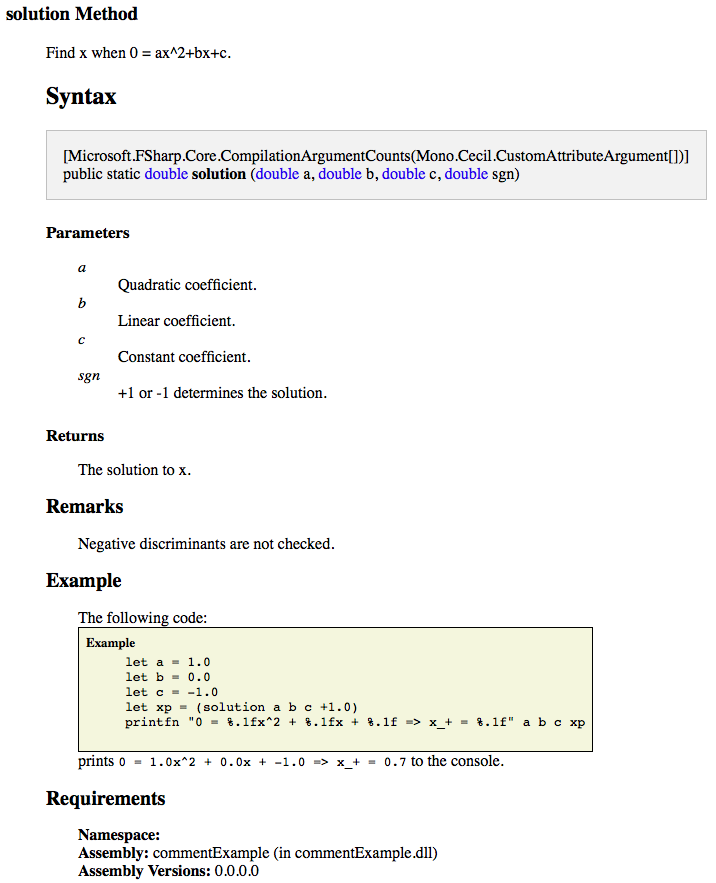
\includegraphics[width=\linewidth]{mdocOutput}
  \caption{Part of the HTML documentation as produced by \lstinline[language=console]{mdoc} and viewed in a browser.}
  \label{fig:htmlDocumentExample}
\end{figure}
A full description of how to use \lstinline[language=console]{mdoc} is found here\footnote{\url{http://www.mono-project.com/docs/tools+libraries/tools/monodoc/generating-documentation/}}.
\end{comment}

Several tools exists which extracts the comments from source code and reorder the comments into manual type structures, such as Doxygen. Popular output from such tools are both HTML and \LaTeX. However, for this text, the usage of the XML-standard as a way to standardize comments will suffice.

\section{Key Concepts and Terms in This Chapter}
This chapter has considered elements that are an important part of the activity of programming, but to some extent complement the specific act of writing source code. You have seen:
\begin{itemize}
\item How to use the \textbf{7-step guide} to design functions, which emphasizes writing examples of function usage before implementing the function itself.
\item Write \textbf{in-code} documentation to support the understanding of the code. 
\item Documentation is written for programmers and there are at least two different types: \textbf{users} and \textbf{maintainers}. 
\item The \textbf{XML standard} uses \lstinline{///}, is for both types of programmers, and documents what a program does and how it is to be used.
\item The \textbf{line} and \textbf{block} comments are for implementation-specific details and intented to be read by programmers who seek to understand and maintain the code. 
\item There is no such thing as the correct documentation, but you are well advised to follow the XML standard and to improve your skill by writing documentation and sharing it with others.
\end{itemize}

\end{document}

